\section{Dataset}

In this section we'll present our dataset and the different steps that were involved in its construction and preparation, we'll also present some statistics about it and compare it to other popular datasets.

\todo[inline]{Showcase some example images from the dataset, or not as we already have done it in the first context section ?}

\subsection{Raw Format}

Our dataset was constructed by filming 10 different climbers attempting to climb 2 different bouldering blocks (events) each. Each climb was filmed from two different angles, resulting in 40 unique videos of 4 mins each.

As specified in the \cite{section:context}, during the bouldering event the boulderer are free to do whatever they want during the 4 minutes, they can brush the holds (grips), observe them, climb, etc. Thus we have 20 climbs and 2 videos for each climb resulting in a total of 40 videos.

The dataset was collected during Manip Chamberry.

Our dataset duration in hours is...

The videos were annotated by the climbers themselves, and the annotations were provided in a raw excel file. The annotations were provided at segment level, meaning that we are given the start and duration of each action in the video and the corresponding label.

From the 20 climbs only 11 are annotated.

Constraints:
- Dataset size is very limited.
- The annotations format (excel) isn't adapted for data science tasks.
- The annotations aren't perfect, they are shifted, and the videos don't start immediately on the event.
- The climbers sometimes go out of the frame, some other times another person enters the frame, etc.

\subsection{Chosen Structure}

We decided to structure the dataset in a way that is adapted for temporal action segmentation and classification tasks. Most importantly, we wanted to make it easy and efficient to use and train on.

\begin{verbatim}
    dataset
    +-- videos
    |   +-- video-1
    |   |   +-- frame-1.jpg
    |   |   +-- frame-2.jpg
    |   |   +-- ...
    |   +-- ...
    +-- annotations
    |   +-- video-1.csv
    |   +-- video-2.csv
    |   +-- ...
    +-- splits
        +-- train.txt
        +-- val.txt
        +-- test.txt
\end{verbatim}

The advantages of this structure is that it don't require any additional video processing on top of the videos or annotations provided by the data collecting team, this makes it very easy and convenient to add annotations or videos in the future if available.

For a faster video loading time we store the video as a sequence of jpg frames rather than the video itself, this also makes it easier to use the dataset with different libraries and tools.

In order to load the dataset we developed a video dataset package in python: \href{https://github.com/raideno/video-dataset}{https://github.com/raideno/video-dataset}. This video-dataset class support this kind of dataset structure but is very customizable and comes with a lot of predefined tools in order to transform an existing dataset into this structure, load videos from video files, load annotations at frame level from text files, etc.

On top of that we also developed another python package: \href{https://github.com/raideno/cached-dataset}{https://github.com/raideno/cached-dataset}. Which is essentially a class that serves as a wrapper around an existing dataset and caches the transformed version of the dataset if any were applied into disk, this is very useful when we want to avoid re-extracting the features each time we train the model and for each epoch.

Using this structure and these tools we were able to easily load the dataset and start training the model on it.

\subsection{Statistics, Illustrations \& Data Exploration}

\begin{figure}[H]
    \centering
    \begin{minipage}{0.245\textwidth}
        \centering
        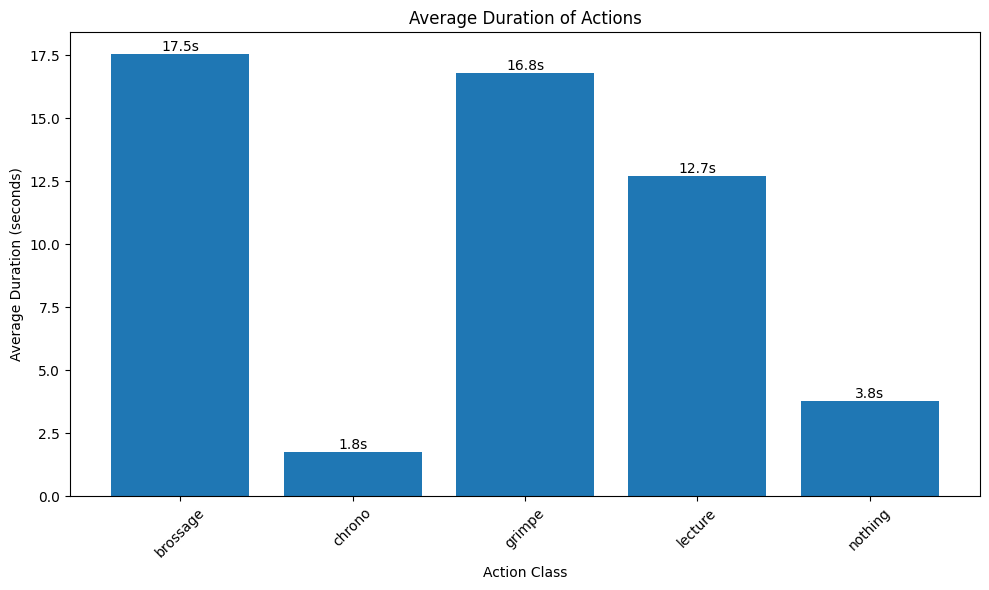
\includegraphics[width=\textwidth]{assets/figures/average-duration-of-actions.png}
        \caption{Statistic 1}
        \label{fig:example1}
    \end{minipage}%
    \hspace{0.02\textwidth} % Spacing between the figures
    \begin{minipage}{0.245\textwidth}
        \centering
        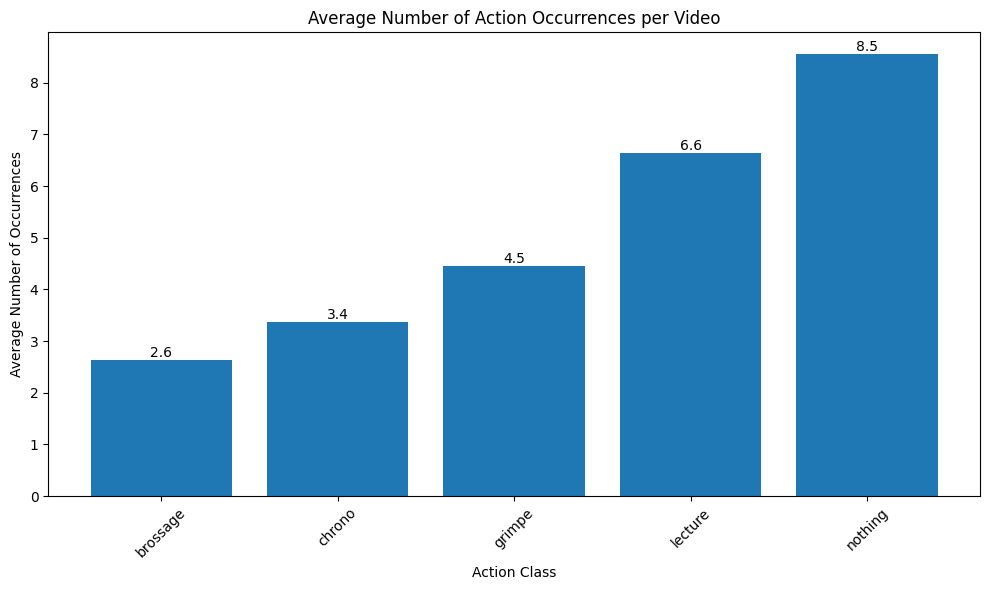
\includegraphics[width=\textwidth]{assets/figures/average-number-of-action-occurences-per-video.png}
        \caption{Statistic 2}
        \label{fig:example2}
    \end{minipage}%
    \hspace{0.02\textwidth} % Spacing between the figures
    \begin{minipage}{0.245\textwidth}
        \centering
        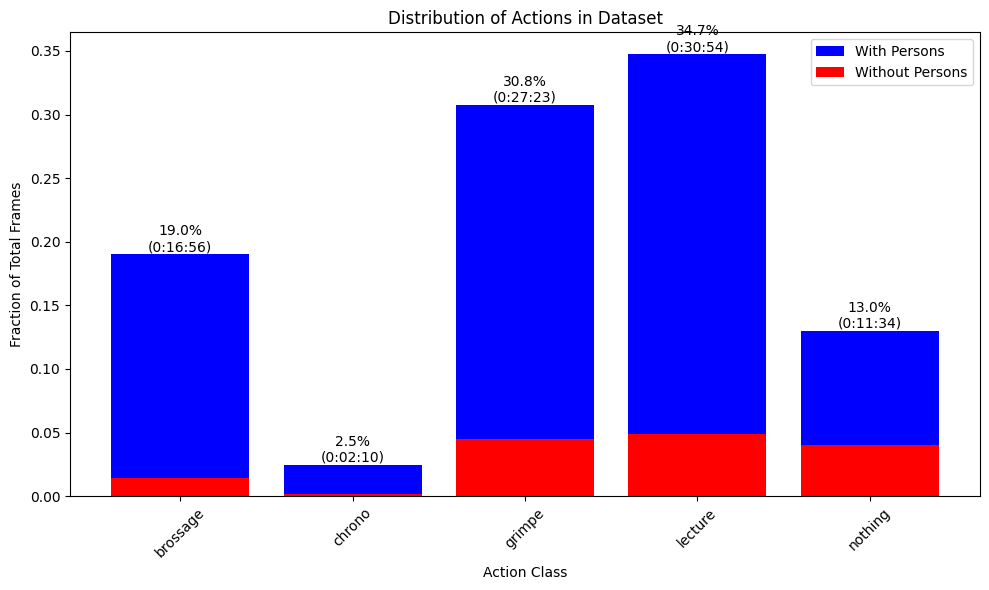
\includegraphics[width=\textwidth]{assets/figures/distribution-of-actions-in-dataset.png}
        \caption{Statistic 3}
        \label{fig:example3}
    \end{minipage}%
\end{figure}

\todo[inline]{Discuss about the statstics above, add the order variation score and the repetitino score...}

\subsection{Other Video Datasets}

\todo[inline]{Add an image from a video of each dataset for illustration.}

\begin{table}[h!]
    \centering
    \begin{tabular}{|l|c|c|c|}
        \hline
        \textbf{Name} & \textbf{\#Classes} & \textbf{\#Videos} & \textbf{Duration (h)} \\ \hline
        50 Salads & 5 & 20 & 3.5 \\ \hline
        GTEA & 8 & 35 & 6.0 \\ \hline
        Breakfasts & 4 & 15 & 2.0 \\ \hline
        Kinetics-400 & 6 & 25 & 4.5 \\ \hline
        Assembly 101 & 6 & 25 & 4.5 \\ \hline
        Howto100M & 6 & 25 & 4.5 \\ \hline
        Something-Something-V2 & 6 & 25 & 4.5 \\ \hline
        \textbf{Ours} & 6 & 25 & 4.5 \\ \hline
    \end{tabular}
    \caption{Other popular datasets.}
    \label{tab:dataset_stats}
\end{table}

When it comes to temporal action segmentation, there is very few datasets available, and the most popular ones are:

\subsection*{50 Salads, Breakfasts, and GTEA Datasets}
These datasets were primarily designed for temporal action segmentation:

\begin{itemize}
    \item \textbf{50 Salads Dataset}: The 50 Salads dataset consists of 50 videos of people preparing salads, with each video lasting between 5 and 10 minutes. The dataset includes 17 distinct actions, with a total duration of 4 hours. The cameras are placed above the kitchen countertop, capturing primarily the interactions of the person's hands with the environment. This setup focuses on fine-grained actions and interactions \cite{50salads-dataset}.
    
    \item \textbf{GTEA Dataset}: The GTEA dataset was introduced in \cite{gtea-dataset}, and it consists of 28 Point of View (POV) videos, where a person is preparing something. Each video contains around 20 sub-actions.
    
    \item \textbf{Breakfasts Dataset}: Introduced in \cite{breakfast-dataset}, this dataset contains 1712 videos of people preparing breakfasts, with the camera positioned on the side.
\end{itemize}

\subsection*{Kinetics Family}
The Kinetics family of datasets is available in three variants: Kinetics-400, Kinetics-600, and Kinetics-700 \cite{kinetics-400-dataset}, \cite{kinetics-600-dataset}, \cite{kinetics-700-dataset}. These datasets are composed of YouTube videos and are annotated with 400, 600, and 700 action classes, respectively. The videos typically last around 10 seconds, and each class contains at least 400 videos. The Kinetics datasets cover a wide variety of video content, focusing on humans performing large-scale tasks (as opposed to fine-grained actions). Originally designed for video classification, Kinetics contains single-labeled video clips.

\subsection*{Assembly101 Dataset}
The Assembly101 dataset, introduced in \cite{assembly101-dataset}, contains 4321 videos of people assembling and disassembling various objects in a factory setting. The cameras are positioned at multiple angles, and some videos are captured from a POV perspective.

\subsection*{HowTo100M Dataset}
Introduced in \cite{howto100m-dataset}, the HowTo100M dataset consists of over 100 million video clips sourced from YouTube and other online platforms. It is a collection of instructional (tutorial) videos covering 23,000 distinct activities.

\subsection*{Something-Something V2}
The Something-Something-V2 dataset, introduced in \cite{something-something-dataset}, includes 220,847 video clips of humans performing basic actions such as picking up a pen. The videos are captured from a POV perspective and are designed for fine-grained action and small interaction tasks.